\documentclass[journal]{IEEEtran}
\usepackage{cite}
\usepackage[cmex10]{amsmath}
\usepackage{url}
\usepackage{graphicx}
\usepackage[latin1]{inputenc}
\usepackage{psfrag}
\usepackage{float,afterpage}
\usepackage{subfig}
\usepackage[linesnumbered,ruled]{algorithm2e}

\newcommand\Real{{\mathbb{R}}}
\newcommand{\vi}{\vspace{0.6\baselineskip}}
\newcommand{\goodgap}{\hspace{\subfigtopskip}\hspace{\subfigbottomskip}}
% Equation
\newcommand{\beq}{\begin{equation}}
\newcommand{\eq}{\end{equation}}
% Equation Array
\newcommand{\beqn}{\begin{eqnarray}}
\newcommand{\eqn}{\end{eqnarray}}
% Bold variables
\newcommand{\mbf}[1]{\ensuremath{\mathbf{#1}}}


\hyphenation{}


\begin{document}
\title{Loudspeaker design model: a toy problem for electromagnetic optimisation}

\author{Felipe~Campelo% <-this % stops a space
\thanks{Operations Research and Complex Systems Laboratory - ORCS Lab, 
Departament of Electrical Engineering, Universidade Federal de Minas Gerais. Contact:{fcampelo@ufmg.br}}}

\markboth{Loudspeaker Design Model}%
{Loudspeaker Design Model}

\maketitle

\IEEEpeerreviewmaketitle


\section{Problem Description}
\IEEEPARstart{T}{he} description of physical characteristics of the loudspeaker device (Figure \ref{fig:ls}) and its optimization are considered in this section. This model is inspired on the loudspeaker design example originally proposed by Infolytica Corporation \cite{infol}. The objective of this problem is the minimization of the total volume of material used, subject to the generation of a given magnetic flux density in the air gap defined by variable $x_9$. Mathematically, the problem is defined as:

\begin{equation}
\begin{array}{ll}\min f\left(\mathbf{x}\right) = $Volume$ \\
$Subject to:$ \left|\mathbf{B}\right| \geq B_{min}\\
\end{array}
\end{equation}

\noindent with $B_{min} = 1.9T$. Of course this problem can also be very easily turned into a multiobjective optimization example, by considering the minimization of volume and the maximization of the magnetic flux density.

Three different materials are considered in this model: \textbf{Air}, \textbf{Pure Iron} and \textbf{Magnet}. The characteristics for each of these materials is given in Table \ref{tab:materials}.

\begin{figure}[htbp]
	\centering
		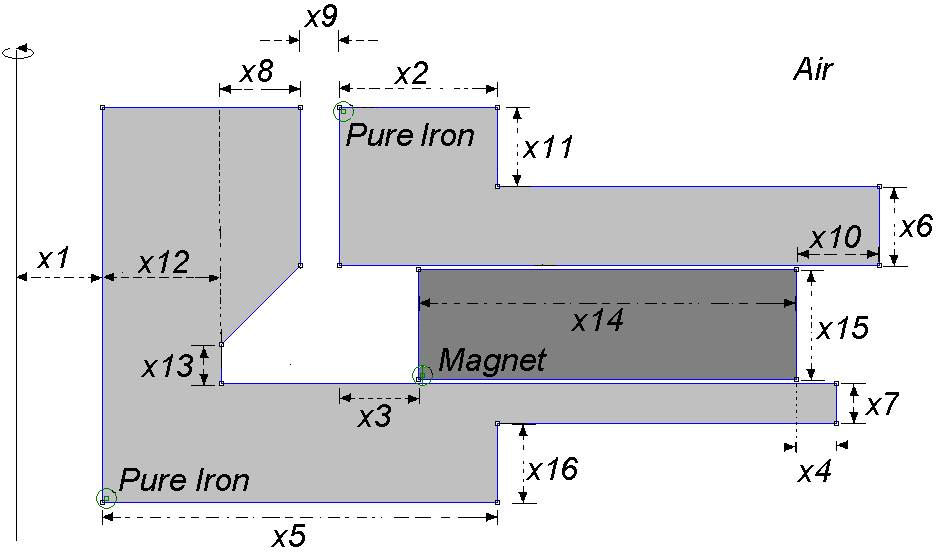
\includegraphics[width=0.45\textwidth]{ls.png}
	\caption{Loudspeaker design model}
	\label{fig:ls}
\end{figure}

\begin{table}[htb]
\caption{Materials Used in the Loudspeaker Model}
\label{tab:materials}
\centering
\begin{tabular*}{8cm}{@{\extracolsep{\fill}}l|cccccc}
\hline
Material Label	& Air		&	Pure Iron	& Magnet\\
\hline
Specification		& Air		& Pure Iron	& NdFeB 40 MGOe magnet\\
$\mu_r$					& 1.0		&	*					&	1.049			\\
$H_c$						& 0.0		& 0.0				&	979,000		\\
$\sigma$				& 0.0		&	10.44			&	0.667			\\
\hline
\end{tabular*}
\end{table}

The nonlinear B-H characteristic for the \textbf{Pure Iron} is modeled by the quadratic interpolation of sample points, as shown in Figure \ref{fig:IronBH}. The data points used to model the nonlinear curve were obtained in the Materials Library of the \textit{FEMM 4.2} finite element solver \cite{femm42}, and are given in Table \ref{tab:IronBH}.

\begin{figure}[htb]
	\centering
		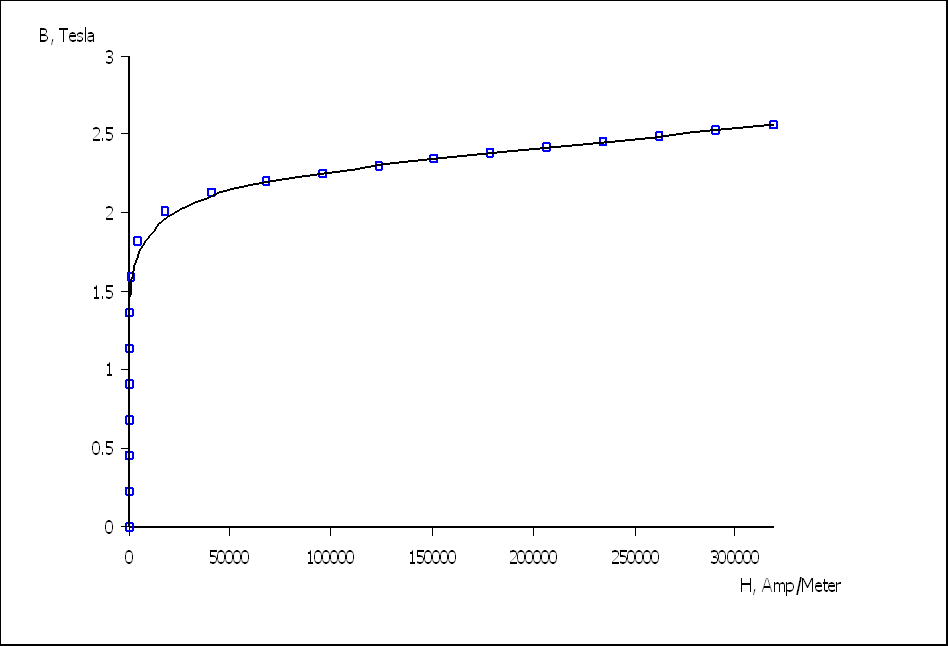
\includegraphics[width=0.45\textwidth]{IronBH.png}
		\caption{B-H curve for the \textbf{Pure Iron}}
	\label{fig:IronBH}
\end{figure}

\begin{center}
\begin{table}[htb]
\caption{Points used for modeling the B-H curve of the \textbf{Pure Iron}}
\label{tab:IronBH}
\centering
\begin{tabular*}{6cm}{@{\extracolsep{\fill}}rc}
\hline
H	[A/m]					& 		B [T]\\
\hline
0.0000 			&   0.0000\\
13.8984 		&   0.2271\\
27.7967 		&   0.4541\\
42.3974 		&   0.6812\\
61.4157 		&   0.9083\\
82.3824 		&   1.1353\\
144.6690		&   1.3624\\
897.7600 		&   1.5894\\
4581.7400 	&   1.8124\\
17736.2000 	&   2.0100\\
41339.3000 	&   2.1332\\
68321.8000 	&   2.2000\\
95685.5000 	&   2.2548\\
123355.0000 &   2.2999\\
151083.0000 &   2.3425\\
178954.0000 &   2.3788\\
206825.0000 &   2.4150\\
234696.0000 &   2.4513\\
262568.0000 &   2.4875\\
290439.0000 &   2.5238\\
318310.0000 &   2.5600\\
\hline
\end{tabular*}
\end{table}
\end{center}

The recommended limits for each design variable are shown in Table \ref{tab:varlims}. This table also provides suggestions of fixed values, used in the case of lower-dimensional formulations of the problem.
\begin{table}[h]
\caption{Limits of the search space}
\label{tab:varlims}
\centering
\begin{tabular*}{8cm}{@{\extracolsep{\fill}}l|cccccc}
\hline
Parameter	&	min		&	max		&	fixed\\
\hline
$x_1$        &$3.0$      	&$12.0$       &$5.0$\\
$x_2$        &$1.0$	     	&$4.0$        &$3.0$\\
$x_3$        &$1.0$	      &$4.0$        &$1.0$\\
$x_4$        &$-1.0$	    &$3.0$        &$0.0$\\
$x_5$        &$5.0$	     	&$15.0$       &$7.0$\\
$x_6$        &$1.0$	     	&$10.0$       &$6.0$\\
$x_7$        &$1.0$	     	&$10.0$       &$2.0$\\
$x_8$        &$3.0$	      &$8.0$        &$5.0$\\
$x_9$        &$0.5$	      &$2.0$        &$0.5$\\
$x_10$       &$-1.0$	    &$3.0$        &$0.0$\\
$x_11$       &$1.0$	      &$7.0$        &$1.0$\\
$x_12$       &$0.05$	  	&$2.0$        &$0.5$\\
$x_13$       &$0.5$	      &$2.0$        &$1.0$\\
$x_14$       &$5.0$	     	&$12.0$       &$7.0$\\
$x_15$       &$1.0$       &$5.0$        &$4.0$\\
$x_16$       &$1.0$	     	&$10.0$       &$1.0$\\
\hline
\end{tabular*}
\end{table}

\section{FEMM model}
The loudspeaker model described above has been implemented using the LUA scripting language \cite{lua}, for use with the Finite Element Method Magnetics (FEMM) v. 4.2 numerical solver \cite{femm42}. The model implemented can handle batch evaluations, and will return an output file containing the values of magnetic flux density and the volume of the device. The FEMM solver can also very easily plot the magnetic field lines and flux density heatmaps. A short tutorial on the FEMM 4.2 solver is available online in \cite{femm42mag}.

\section{How to use the model}
\begin{enumerate}
\item Required Software:
\begin{itemize}
\item Finite Element Method Magnetics v.4.2
\item Matlab (not \textit{really} required, but some Matlab routines are provided)
\end{itemize}
\item Required files \cite{files}:
\begin{itemize}
\item loudspeaker.lua
\item CallFEMM\_LS.m
\item LS\_fun.m
\end{itemize}
\item Problem options:
\begin{itemize}
\item Full model (16 vari�veis)
\item Partial model (7 variables):\begin{itemize}
\item[] $\left[x_{2},\ x_{6},\ x_{9},\ x_{10},\ x_{11},\ x_{14},\ x_{15}\right]$\end{itemize}
\end{itemize}
\item How to use:
\begin{itemize}
\item Copy all files contained in \cite{files}  in a local folder (e.g., 'C:$\backslash$loudspeaker$\backslash$')
\item Enter the correct path in lines 33-35 of file \textit{loudspeaker.lua}. Attention to the old-windows style of treating long names or names with spaces.
\item Enter the correct path in 5-8 of \textit{CallFEMM\_LS.m}. Attention to the old-windows style of treating long names or names with spaces.
\end{itemize}
\end{enumerate}

\subsection{Testing the model}
You can verufy if the model is working by:
\begin{enumerate}
\item LUA script:
\begin{itemize}
\item Open 4.2;
\item Select \textit{File - Open LUA Script - loudspeaker.lua}
\item If \textit{loudspeaker.lua} is correct, FEMM will execute a test simulation (defined by input file \textit{loudspeaker.in} in \cite{files}) and close automatically.\\
\end{itemize}
\item \textit{CallFEMM\_LS.m}:
\begin{itemize}
\item Open Matlab and select the folder containing the loudspeaker files;
\item On the console, type:\\
$>>$ X = [5.0,3.0,1.0,0.0,7.0,6.0,2.0,5.0,0.5,...\\
0.0,1.0,0.5,1.0,7.0,4.0,1.0]';\\
$>>$ Y = CallFEMM\_LS(X)
\item If your path is correct, the FEMM 4.2 window should pop up in your screen, run the dummy simulation, and return the result:\\
Y =\\
    0.5272\\
    0.0000\\
    0.0000
    
The following call:\\
$>>$ F = LS\_fun(X)

\noindent should then yield the penalized objective function value:\\
F =\\
  159.5294
  \end{itemize}
\end{enumerate}


Besides function \textit{LS\_fun.m}, the routines \textit{LS\_vol.m} and \textit{LS\_B.m} can be useful, since they return the volume and magnetic flux density values separately. The Matlab routines and the LUA script are all extensively commented, and can be easily adapted for a wide range of optimization routines.

\section{Maiores informa��es}
Questions, bug reports, comments and suggestions can be filed to \cite{files}, or sent directly to \url{fcampelo@ufmg.br}.


\begin{thebibliography}{1}
\bibitem{infol}
{Infolytica Corporation},
``Optimization - Minimizing Loudspeaker Mass'',
\emph{online}, available from: \url{http://www.infolytica.com/en/applications/ex0086/}

\bibitem{femm42}
David Meeker,
``Finite Element Method Magnetics, v. 4.2'',
\emph{online}, available from: \url{http://www.femm.info/wiki/HomePage}

\bibitem{lua}
R. Ierusalimschy, L. H. de Figueiredo, W. Celes,
``LUA scripting language'',
\emph{online}, available from: \url{http://www.lua.org/}

\bibitem{femm42mag}
David Meeker,
``Finite Element Method Magnetics v. 4.2 - Magnetics tutorial'',
\emph{online}, available from: \url{http://www.femm.info/Archives/doc/tutorial-magnetic.pdf}

\bibitem{files}
Felipe Campelo,
``Loudspeaker design model'',
\emph{online}, available from: \url{https://github.com/fcampelo/Loudspeaker-model}

\end{thebibliography}



% that's all folks
\end{document}


